% 华东师范大学博士(硕士)论文主格式,请修改前三行以保证格式符合要求。

%==============格式配置开始==============%
\def \degree {phd} % phd, master
\def \year {2025}
\def \draftfigure {off} % on,off
\def \docstyle {normal} % normal,tmlc,anonymous
\def \refstyle {auto} % auto,manual

% student id
\def \stuID {52xxxxxx}
% title
\def\thesisTitle{论文标题}
\def\thesisTitleNoWrap{论文标题}
\def\thesisETitle{
    Title
}
%==============格式配置结束==============%

\def \dc {on}
\ifx \draftfigure \dc
\documentclass[12pt,a4paper,fancyhdr,openany,twoside,draft]{ctexbook}
\else
\documentclass[12pt,a4paper,fancyhdr,openany,twoside]{ctexbook}
\fi

\def \phd {phd}
\ifx \degree \phd
    \def\degreeCN{博士}
    \def\degreeENs{Doctoral}
\else
    \def\degreeCN{硕士}
    \def\degreeENs{Master's}
\fi

\usepackage[CJKbookmarks,
colorlinks,
linkcolor=black,
anchorcolor=black,
citecolor=black,
urlcolor=black
]{hyperref}
\usepackage{shortvrb,ulem,makeidx}
\usepackage{fancyhdr}
\usepackage{graphicx}
\usepackage{indentfirst,latexsym,colortbl,subfigure,clrscode}
\usepackage{algorithm}
\usepackage{algorithmic}
\usepackage{bm}                     % 处理数学公式中的黑斜体的宏包
\usepackage{amsmath}                % AMSLaTeX宏包 用来排出更加漂亮的公式
\usepackage{amssymb}                % AMSLaTeX宏包 用来排出更加漂亮的公式
\usepackage{mathrsfs}
\usepackage[subnum]{cases}
% \usepackage[numbers]{natbib} %sort&compress
\usepackage{geometry}
\usepackage{url}
\usepackage{times}
\usepackage{fontspec}
\usepackage{makecell,rotating,multirow,diagbox}
\usepackage{booktabs}
\usepackage{caption}
\usepackage{titletoc}
\usepackage{amsthm}
\usepackage{fourier} 
\usepackage{mathtools}

\urlstyle{same} %使用\url{}以开启链接的自动换行,该命令保证超链接文本字体样式与正文一致

\newcommand\cplus{\mathbin{\raisebox{-\height}{$+$}}}
\newcommand\contdots{\raisebox{-\height}{$\vphantom{+}\dotsm$}}
\newtheorem{hypothesis}{假设}[chapter]
\newif\ifnotanonymous\notanonymoustrue		%定义是否开启盲审,默认不开启
\newif\iftmlc

\def\cFracB#1#2{%
	\vcenter{\hbox{\strut$#1$\,\vrule}\hrule\hbox{\strut\vrule\,$#2$}}}
\makeindex
\pagestyle{fancy}

\renewcommand{\headrulewidth}{0.4pt}
\fancyfoot[RO,LE]{\thepage}
\fancyfoot[CO,CE]{}
\renewcommand{\algorithmicrequire}{\textbf{Input:}}
\renewcommand{\algorithmicensure}{\textbf{Output:}}
\newcommand{\loflabel}{图}
\newcommand{\lotlabel}{表}
\captionsetup[table]{labelsep=quad}
\captionsetup[figure]{labelsep=quad}


%                    根据自己正文需要做的一些定义                 %
%==================================================================%
\def\diag{{\rm diag}}
\def\rank{{\rm rank}}
\def\RR{{\cal R}}
\def\NN{{\cal N}}
\def\R{{\mathbb R}}
\def\C{{\mathbb C}}
\let\dis=\displaystyle

\def\p{\partial}
\def\f{\frac}
\def\mr{\mathrm}
\def\mb{\mathbf}
\def\mc{\mathcal}
\def\b{\begin}
\def\e{\end}

\newtheorem{thm1}{Theorem}[part]
\newtheorem{thm2}{Theorem}[section]
\newtheorem{thm3}{Theorem}[subsection]
\newtheorem{them}[thm2]{定理}
\newtheorem{theorem}[thm2]{定理}
\newtheorem{defn}[thm2]{定义}
\newtheorem{define}[thm2]{定义}
\newtheorem{ex}[thm2]{例}
\newtheorem{exs}[thm2]{例}
\newtheorem{example}[thm2]{例}
\newtheorem{prop}[thm2]{命题}
\newtheorem{lemma}[thm2]{引理}
\newtheorem{cor}[thm2]{推论}
\newtheorem{remark}[thm2]{注释}
\newtheorem{notation}[thm2]{记号}
\newtheorem{abbre}[thm2]{缩写}
% \newtheorem{algorithm}[thm2]{算法}
\newtheorem{problem}[thm2]{问题}
\newtheorem{Definition}{定义}[chapter]


\newcommand{\cyihao}{\fontsize{26pt}{30pt}\selectfont}			% 一号, 1.5 倍行距
\newcommand{\yihao}{\fontsize{26pt}{36pt}\selectfont}			% 一号, 1.4 倍行距
\newcommand{\erhao}{\fontsize{22pt}{28pt}\selectfont}			% 二号, 1.25倍行距
\newcommand{\xiaoer}{\fontsize{18pt}{18pt}\selectfont}          % 小二, 单倍行距
\newcommand{\sanhao}{\fontsize{16pt}{24pt}\selectfont}			% 三号, 1.5倍行距
\newcommand{\xiaosan}{\fontsize{15pt}{22pt}\selectfont}			% 小三, 1.5倍行距
\newcommand{\sihao}{\fontsize{14pt}{21pt}\selectfont}			% 四号, 1.5 倍行距
\newcommand{\banxiaosi}{\fontsize{13pt}{19.5pt}\selectfont}		% 半小四, 1.5倍行距
\newcommand{\xiaosi}{\fontsize{12pt}{18pt}\selectfont}			% 小四, 1.5倍行距
\newcommand{\dawuhao}{\fontsize{11pt}{11pt}\selectfont}			% 大五号, 单倍行距
\newcommand{\wuhao}{\fontsize{10.5pt}{15.75pt}\selectfont}		% 五号, 单倍行距

%============================ 可以自定义文字块 ================================%

\newcommand{\aaa}{Example}
\newcommand{\bbb}{\aaa \aaa \aaa}
\newcommand{\ccc}{\bbb \bbb \bbb \bbb \bbb
	
	\bbb \bbb \bbb \bbb \bbb }
\newcommand{\abc}{abcdefg1234567890}
\newcommand{\upabc}{ABCDEFGHIJK}
%%% ----------------------------------------------------------------------

\CTEXsetup[beforeskip = 0pt]{chapter}
\CTEXsetup[afterskip = 20pt]{chapter}


%============================= 版芯控制 ================================%
\setlength{\oddsidemargin}{0.57cm} 
\setlength{\evensidemargin}{\oddsidemargin}
\voffset-6mm \textwidth=150mm \textheight=230mm \headwidth=150mm
%\rightmargin=35mm
%                                                                       %


%============================= 页面设置 ================================%
%-------------------- 定义页眉和页脚 使用fancyhdr 宏包 -----------------%
% 定义页眉与正文间双隔线
%my addition
\fancyhead{}
\fancyhead[RO,LE]{\bfseries 华东师范大学{\degreeCN}学位论文}
\fancyhead[LO,RE]{\small\leftmark}
%end myaddition

\newcommand{\makeheadrule}{%
	\makebox[0pt][l]{\rule[.7\baselineskip]{\headwidth}{0.4pt}}%
	\rule[0.85\baselineskip]{\headwidth}{0.4pt} \vskip-.8\baselineskip}
\makeatletter
\renewcommand{\headrule}{%
	{\if@fancyplain\let\headrulewidth\plainheadrulewidth\fi
		\makeheadrule}} \makeatother

\newcommand{\adots}{\mathinner{\mkern 2mu%
		\raisebox{0.1em}{.}\mkern 2mu\raisebox{0.4em}{.}%
		\mkernmu\raisebox{0.7em}{.}\mkern 1mu}}
\renewcommand{\contentsname}{\heiti \sanhao {目\quad 录}}
\renewcommand{\listfigurename}{\heiti \sanhao {图目录}}
\renewcommand{\listtablename}{\heiti \sanhao {表目录}}
\setmainfont{Times New Roman}
\dottedcontents{chapter}[1.5cm]{\sihao\heiti}{3.8em}{9.5pt}
\dottedcontents{section}[1.5cm]{\xiaosi\heiti}{2.8em}{9.5pt}
\DeclareRobustCommand\nobreakspace{\leavevmode\nobreak\ }




%============================= Bibitem control ================================% 
\def \auto {auto}
\ifx \refstyle \auto

\else

\usepackage{etoolbox} % Required, for availablility changing the latex env.
% \usepackage{hyperref} % Show a green-border box on each \cite label?

% Pre-define list variables
\makeatletter
\newcommand*{\lodbib@citeorder}{} % Catch normal entries
\newcommand*{\lodbib@notcited}{} % Catch entries that were not cited

% Macro in aux file
\def\citation{%
  \forcsvlist{\citation@i}}

\def\citation@i#1{%
  \ifinlist{#1}{\lodbib@citeorder}
    {}
    {\listxadd{\lodbib@citeorder}{#1}}}

\let\ltxorig@lbibitem\@lbibitem
\let\ltxorig@bibitem\@bibitem

% Save bibitems into lists
\def\@lbibitem[#1]#2#3{%
  \csdef{lodbib@savedlabel@#2}{#1}%
  \@bibitem{#2}{#3}}

\def\@bibitem#1#2{%
  \xifinlist{#1}{\lodbib@citeorder}
    {}
    {\listadd{\lodbib@notcited}{#1}}%
  \csdef{lodbib@savedentry@#1}{#2}}

% Re-define \thebibiography command.
\renewenvironment{thebibliography}[1]
     {\settowidth\labelwidth{\@biblabel{#1}}}
     {\def\@noitemerr
       {\@latex@warning{Empty `thebibliography' environment}}%
      \chapter*{参考文献} % chapter title
       \@mkboth{参考文献}{参考文献} % left page header / right page header
      \list{\@biblabel{\@arabic\c@enumiv}}%
           {\leftmargin\labelwidth\parsep=0pt
            \advance\leftmargin\labelsep
            \@openbib@code
            \usecounter{enumiv}%
            \let\p@enumiv\@empty
            \renewcommand\theenumiv{\@arabic\c@enumiv}}%
      \sloppy
      \clubpenalty4000
      \@clubpenalty \clubpenalty
      \widowpenalty4000%
      \sfcode`\.\@m
      \lodbib@biblistloop
      \endlist}
      
% Output the bib list.
\def\lodbib@biblistloop{%
  \forlistloop{\lodbib@bibitem}{\lodbib@citeorder}%
  \ifdefvoid{\lodbib@notcited}
    {}
    {\forlistloop{
    \lodbib@bibitem 
    }{
    %\lodbib@notcited % Whether listing uncited bib at the end of the references?
    }}}
    
% Modify the \cite num. in the book.
\def\lodbib@bibitem#1{%
  \ifcsundef{lodbib@savedlabel@#1}
    {\ltxorig@bibitem{#1}}
    {\ltxorig@lbibitem[\csuse{lodbib@savedlabel@#1}]{#1}}%
  \csuse{lodbib@savedentry@#1}}
  

\fi
 

%============== Convert all headers (incl. bib sec.) and footers into fancy style, with double underlines and book titles adding to the headers, pages num. adding to the footers.========%
\makeatletter
\let\ps@plain\ps@fancy

\usepackage{enumitem}
\setenumerate{itemsep=0pt,partopsep=0pt,parsep=\parskip,topsep=0pt}
\setitemize{itemsep=5pt,partopsep=0pt,parsep=\parskip,topsep=10pt,leftmargin=25pt,labelsep=10pt}
% \setdescription{itemsep=0pt,partopsep=0pt,parsep=\parskip,topsep=0pt}


%======================= TOC Settings =======================%
\titlecontents{chapter}[4.5em]{\sihao\heiti}%最前面到标题的缩进
              {\contentslabel{4em}}%序号和标题文字之间的缩进
              {\hspace{-4em}}%无序号标题往前缩进
              {\ \titlerule*[0.4pc]{$\cdot$}\contentspage}{} %引导线为"...1"
\titlecontents{section}[4.5em]{\heiti \xiaosi}%最前面到标题的缩进
              {\contentslabel{2.5em}}%序号和标题文字之间的缩进
              {}%
              {\ \titlerule*[0.4pc]{$\cdot$}\contentspage}{} %引导线为"...1"
\titlecontents{subsection}[7.5em]{}%最前面到标题的缩进
              {\contentslabel{2.9em}}%序号和标题文字之间的缩进
              {}%
              {\ \titlerule*[0.4pc]{$\cdot$}\contentspage}{} %引导线为"...1"
\titlecontents{figure}[0em]{}%最前面到标题的缩进
              {\figurename~\thecontentslabel \quad}%序号和标题文字之间的缩进
              {}%
              {\ \titlerule*[0.4pc]{$\cdot$}\contentspage}{} %引导线为"...1"
\titlecontents{table}[0em]{}%最前面到标题的缩进
              {表~\thecontentslabel \quad}%序号和标题文字之间的缩进
              {}%
              {\ \titlerule*[0.4pc]{$\cdot$}\contentspage}{} %引导线为"...1"

% Activate all \makeatletter script
\makeatother

\def \dd {anonymous}
\def \de {tmlc}
\ifx \docstyle \dd
    \notanonymousfalse % 开启该行则为盲审版本,注释该行则为非盲审版本(即查重或终稿版本)
\else
    \ifx \docstyle \de
        \tmlctrue % 开启该行则为查重版本,注释该行则为终稿版本(仅在上一行在注释状态下有效)
    \fi
\fi

% 以下是正文部分

\usepackage{emptypage}
\usepackage{tikz}
\usepackage{bbm}
%	\usepackage{algorithm}
\usepackage{multirow}
\usepackage{bbm}
% \usepackage{algpseudocode}
\usepackage{wrapfig}
\usepackage{graphicx}
\usepackage{subfigure}
\usepackage{array} % Necessary for new column definitions
\usepackage{listings}
% Define \tabincell
\newcommand\tabincell[2]{\begin{tabular}{@{}#1@{}}#2\end{tabular}}
%\usepackage{algorithm,algpseudocode}
\usepackage{lipsum}
%\usepackage{algorithmic}
%\usepackage{subcaption}
\usepackage{amsfonts}
\usepackage{xcolor}
\newtheorem{Proposition}{Theorem}
\DeclareMathOperator*{\argmax}{arg\,max}
\DeclareMathOperator*{\argmin}{arg\,min}
\newtheorem{proposition}{Proposition}
\theoremstyle{definition}
\newtheorem{definition}{Definition}
\newtheorem{assumption}{Assumption}
\theoremstyle{remark}
\usepackage{enumitem}
\usepackage{pifont}
\usepackage{xspace}
\newcommand{\greencheck}{{\checkmark}}
\newcommand{\xmark}{\ding{55}}%
% \newcommand{\redx}{{\color{red}\xmark}}
\newcommand{\redx}{{\xmark}}
% \usepackage{algorithmic}

\usepackage{xeCJK} % 声明包
%\renewcommand{\algorithmcfname}{算法}
\floatname{algorithm}{算法}
\renewcommand{\algorithmicrequire}{\textbf{输入:}}
\renewcommand{\algorithmicensure}{\textbf{输出:}}
\begin{document}
\pagestyle{empty}
\setlength{\baselineskip}{25pt}  %%正文设为25磅行间距
\vspace{-2.0cm}
\noindent{{\zihao{4} {\large \year} 届研究生{\degreeCN}学位论文}}\\
\vspace{-0.8cm}
\begin{flushleft}
\hspace{-0.5cm}
\renewcommand\arraystretch{1.5}
\begin{tabular}{l}
    \noindent{{\zihao{4} 分类号:\underline{~~~\qquad\qquad\qquad\qquad}}}   \\
    \noindent{{\zihao{4} 密~~~~级:\underline{~~~\qquad\qquad\qquad\qquad}}} \\
\end{tabular}
\hskip 1.1cm
\renewcommand\arraystretch{1.5}
\begin{tabular}{l}
    \noindent{{\zihao{4} 学校代码:\underline{~~~\qquad 10269 \qquad~~~}}}   \\  %10269
    \noindent{{\zihao{4} 学~~~~~~~~号:\underline{~~~~~~{\ifnotanonymous \stuID \else *********** \fi}~~~~~}}} \\
\end{tabular}
\end{flushleft}


\vskip 1.3cm

\begin{center}
% \hskip 0.2cm
% \scalebox{1.0}{\includegraphics[width=2.7cm]{chapters/fig-0/ecnulogo.png}}
\scalebox{1.0}{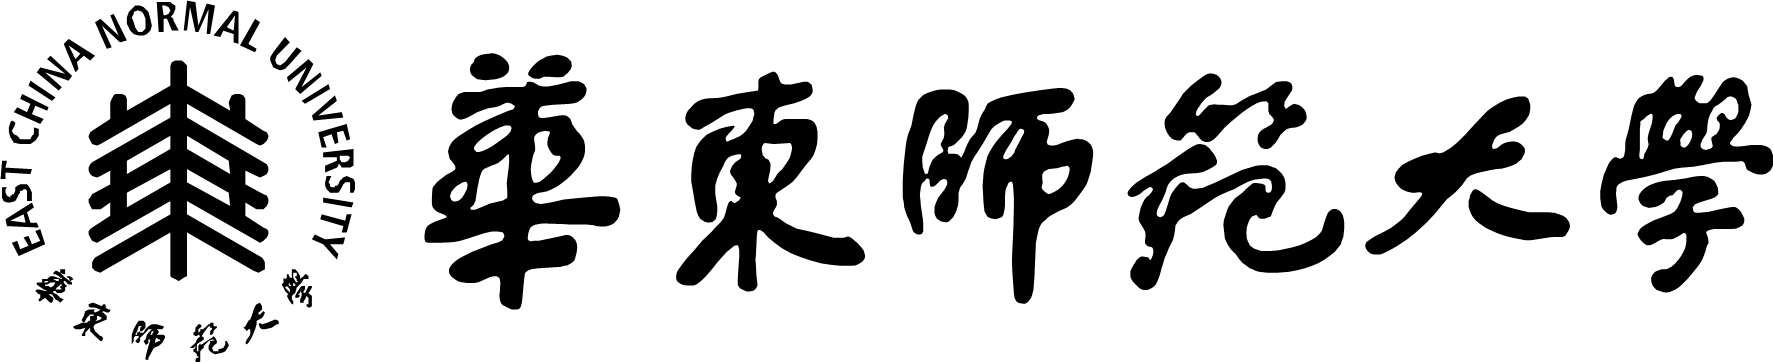
\includegraphics[width=13.2cm]{chapters/figs/logo.png}}
\vskip 0.5cm
{{\xiaosi East China Normal University}}\\ 
{\textbf{\xiaosi {\degreeCN}学位论文}}\\ 
{\textbf{{\xiaosi \MakeUppercase{\degreeENs} DISSERTATION}}}\\
\end{center}

\vskip 0.8cm % 1.0cm

\begin{center}
{\yihao \bf {\thesisTitle}}
% {\cyihao \bf 论文题目:\underline{论文格式研究与} \par }
% {\cyihao \bf \underline{更长的标题编写} \par }
%{\erhao \bf ~~~~\underline{}
\end{center}

\newcommand{\coverlength}{2.7cm}
\vskip 1.0cm 
\begin{center}
    \renewcommand\arraystretch{1.5}
    \begin{tabular}{l}
        \makebox[\coverlength][s]{\sihao \bf 院系:}~~\\
        \makebox[\coverlength][s]{\sihao \bf 专业:}\\ 
        \makebox[\coverlength][s]{\sihao \bf 研究方向:}\\
        \makebox[\coverlength][s]{\sihao \bf 指导教师:}\\ 
        \makebox[\coverlength][s]{\sihao \bf 学位申请人:}
    \end{tabular}
    \begin{tabular}c
        {\sihao \bf ~~~xxxx~~~}\\ 
        \hline {\sihao \bf xxx}\\ 
        \hline {\sihao \bf xxx}\\ 
        \hline {\sihao \bf \ifnotanonymous ~~xxx~~副教授~~ ~~xxx~~教授~~ \else *** \fi}\\
        \hline{\sihao \bf  \ifnotanonymous ~~xxx~~ \else *** \fi}\\
        \hline
    \end{tabular}
\end{center}

\vskip 3.5cm 

\begin{center}
    {\sihao {2024}年11月x日}
\end{center}

\cleardoublepage
\newpage

\pagestyle{empty}

\noindent{\large Dissertation for {\degreeENs} Degree in {\year}}\\
\hspace*{\fill} {\large University Code: 10269}\\
\hspace*{\fill} {\large Student ID: \ifnotanonymous \stuID \else *********** \fi}

\vskip 2cm

\begin{center}
    {\Huge $\mathbb{EAST}\,\mathbb{CHINA}\,\mathbb{NORMAL}\,
            \mathbb{UNIVERSITY}$}
\end{center}

\vskip 3cm

\begin{center}
    \bfseries{\scshape{\huge {\thesisETitle}}} \\
\end{center}

\vskip 2cm

{\large
\begin{center}
\begin{tabular}{r}
    Department:         \\
    % \\
    Major:              \\
    Research Direction: \\
    Supervisor:         \\ 
    Candidate:
\end{tabular}
\begin{tabular}c
    % 盲审需要注释下面一些信息,注意页面上的学号是否需要注释

    School of xxx \\
    \hline xxx \\
    \hline  xxx  \\
    \hline \ifnotanonymous A/Prof. xxx \ \ Prof. xxx \else *** \fi \\ %Prof. Xiaoling Wang  \\
    \hline \ifnotanonymous xxx \else *** \fi \\
    % ~~~~~~~~~~~~~~~~~~~~~~~~~~~~~~~~~        \\
    % \hline ~~~~~~~~~~~~~~~~~~~~~~~~~~~~~~~~~ \\
    % \hline ~~~~~~~~~~~~~~~~~~~~~~~~~~~~~~~~~ \\
    % \hline ~~~~~~~~~~~~~~~~~~~~~~~~~~~~~~~~~ \\
    % \hline ~~~~~~~~~~~~~~~~~~~~~~~~~~~~~~~~~ \\

    \hline
\end{tabular}
\end{center}
}


\vskip 5cm  

\begin{center}
    {\Large November, 2024}
\end{center}

\cleardoublepage

\ifnotanonymous %非盲审,也就是查重版,不显示原创性+名单;终版全要
    \iftmlc
    \else
        \newpage
\pagestyle{empty}
\centerline{\bf\Large 华东师范大学学位论文原创性声明}

\vskip 1cm

\normalsize \indent
郑重声明:本人呈交的学位论文《{\thesisTitleNoWrap}》,是在华东师范大学攻读硕士/博士(请勾选)学位期间,在导师的指导下进行的研究工作及取得的研究成果。除文中已经注明引用的内容外,本论文不包含其他个人已经发表或撰写过的研究成果。对本文的研究做出重要贡献的个人和集体,均已在文中作了明确说明并表示谢意。
% $$\\  $$
\vskip 1cm

\qquad {作者签名}:$\underline{\qquad\qquad\qquad\qquad }$
\qquad\qquad \qquad \mbox {日期}: ~~\qquad 年 \qquad 月 \qquad 日


\vskip 1cm

\centerline{\bf\Large 华东师范大学学位论文著作权使用声明}

\vskip 1cm

《{\thesisTitleNoWrap}》系本人在华东师范大学攻读学位期间在导师指导下完成的硕士/博士(请勾选)学位论文,本论文的研究成果归华东师范大学所有。本人同意华东师范大学根据相关规定保留和使用此学位论文,并向主管部门和相关机构如国家图书馆、中信所和“知网”送交学位论文的印刷版和电子版;允许学位论文进入华东师范大学图书馆及数据库被查阅、借阅;同意学校将学位论文加入全国博士、硕士学位论文共建单位数据库进行检索,将学位论文的标题和摘要汇编出版,采用影印、缩印或者其它方式合理复制学位论文。

本学位论文属于(请勾选)

(\quad)1.经华东师范大学相关部门审查核定的“内部”或“涉密”学位论文*,
于 ~\qquad 年 \qquad 月 \qquad 日解密,解密后适用上述授权。

(\quad)2.不保密,适用上述授权。
% $$\\ $$
\vskip 0.5cm

\qquad \mbox{导师签名}:$\underline{\qquad\qquad\qquad\qquad}$
\qquad\qquad \mbox {本人签名}:$\underline{\qquad\qquad\qquad\qquad }$

\vskip 0.5cm

$\rightline{ \qquad 年 \qquad  月 \qquad  日 \qquad}$

\vskip 0.5cm

* “涉密”学位论文应是已经华东师范大学学位评定委员会办公室或保密委员会审定过的学位论文(需附获批的《华东师范大学研究生申请学位论文“涉密”审批表》方为有效),未经上述部门审定的学位论文均为公开学位论文。此声明栏不填写的,默认为公开学位论文,均适用上述授权)。
 
        \cleardoublepage
        %\newpage
\pagestyle{empty}
$$\\ \\ \\ $$

\centerline{\bf\Large ${\mbox{\kaishu { }}}\,\,${\degreeCN}学位论文答辩委员会成员名单}


\vskip 10mm

\begin{center}
{
\renewcommand{\arraystretch}{1.75}
\large
\begin{tabular}{| m{25mm}<{\centering}| m{25mm}<{\centering}| m{45mm}<{\centering}| m{25mm}<{\centering}|}\hline 
 {\heiti 姓名}&{\heiti 职称} & {\heiti 单位} &{\heiti 备注}  \\\hline
 
  & & & {\heiti 主席}\\\hline
  & & & {\heiti }\\\hline
 & & & {\heiti }\\\hline
 & & & {\heiti }\\\hline
  & & & {\heiti }\\\hline

\end{tabular}
}
\end{center}

       % \cleardoublepage
    \fi
\else %盲审仅显示原创性,不要名单
    \newpage
\pagestyle{empty}
\centerline{\bf\Large 华东师范大学学位论文原创性声明}

\vskip 1cm

\normalsize \indent
郑重声明:本人呈交的学位论文《{\thesisTitleNoWrap}》,是在华东师范大学攻读硕士/博士(请勾选)学位期间,在导师的指导下进行的研究工作及取得的研究成果。除文中已经注明引用的内容外,本论文不包含其他个人已经发表或撰写过的研究成果。对本文的研究做出重要贡献的个人和集体,均已在文中作了明确说明并表示谢意。
% $$\\  $$
\vskip 1cm

\qquad {作者签名}:$\underline{\qquad\qquad\qquad\qquad }$
\qquad\qquad \qquad \mbox {日期}: ~~\qquad 年 \qquad 月 \qquad 日


\vskip 1cm

\centerline{\bf\Large 华东师范大学学位论文著作权使用声明}

\vskip 1cm

《{\thesisTitleNoWrap}》系本人在华东师范大学攻读学位期间在导师指导下完成的硕士/博士(请勾选)学位论文,本论文的研究成果归华东师范大学所有。本人同意华东师范大学根据相关规定保留和使用此学位论文,并向主管部门和相关机构如国家图书馆、中信所和“知网”送交学位论文的印刷版和电子版;允许学位论文进入华东师范大学图书馆及数据库被查阅、借阅;同意学校将学位论文加入全国博士、硕士学位论文共建单位数据库进行检索,将学位论文的标题和摘要汇编出版,采用影印、缩印或者其它方式合理复制学位论文。

本学位论文属于(请勾选)

(\quad)1.经华东师范大学相关部门审查核定的“内部”或“涉密”学位论文*,
于 ~\qquad 年 \qquad 月 \qquad 日解密,解密后适用上述授权。

(\quad)2.不保密,适用上述授权。
% $$\\ $$
\vskip 0.5cm

\qquad \mbox{导师签名}:$\underline{\qquad\qquad\qquad\qquad}$
\qquad\qquad \mbox {本人签名}:$\underline{\qquad\qquad\qquad\qquad }$

\vskip 0.5cm

$\rightline{ \qquad 年 \qquad  月 \qquad  日 \qquad}$

\vskip 0.5cm

* “涉密”学位论文应是已经华东师范大学学位评定委员会办公室或保密委员会审定过的学位论文(需附获批的《华东师范大学研究生申请学位论文“涉密”审批表》方为有效),未经上述部门审定的学位论文均为公开学位论文。此声明栏不填写的,默认为公开学位论文,均适用上述授权)。
 %查重不显示
    \cleardoublepage %查重不显示
\fi

\setlength{\baselineskip}{25pt}  %正文设为25磅行间距
\newpage
\pagenumbering{roman}
\pagestyle{plain}

\chapter*{\xiaosan\heiti{摘\quad 要}}
\addcontentsline{toc}{chapter}{摘要}
摘要内容

摘要内容

摘要内容

\vspace{0.5cm}
% \hspace{-1cm}
\sihao{\heiti{关键词:}}\xiaosi{关键词1,关键词2,关键词3,关键词4,关键词5}


\cleardoublepage
\newpage
\vspace{-1cm}
\chapter*{\zihao{-3}\heiti{ABSTRACT}}
\addcontentsline{toc}{chapter}{Abstract}
\vspace{-0.5cm}

Abstract content

Abstract content

Abstract content

\vspace{0.5cm}
\hspace{-1cm}
{\bf{\sihao{Keywords:}}} \textit{keywords1, keywords2, keywords3, keywords4, keywords5}






































\cleardoublepage

\setcounter{tocdepth}{2}
\tableofcontents
\cleardoublepage
% \renewcommand{\listfigurename}{\heiti \xiaosan 图目录}
% \renewcommand{\listtablename}{\heiti \xiaosan 表目录} 
\renewcommand{\numberline}[1]{\loflabel~#1\hspace*{1em}}
%设置图目录编号样式,主要是间距
\addcontentsline{toc}{chapter}{图目录}
\listoffigures
%自动生成图目录
\cleardoublepage

% 表格目录
\renewcommand{\numberline}[1]{\lotlabel~#1\hspace*{1em}}
\addcontentsline{toc}{chapter}{表目录}
\listoftables

\cleardoublepage

\newpage
\pagenumbering{arabic}
\pagestyle{fancy}

\CTEXsetup[format+={\zihao{3}\heiti}]{chapter}
\CTEXsetup[format+={\raggedright\zihao{4}\heiti}]{section}
\CTEXsetup[format+={\zihao{-4}\heiti}]{subsection}


\chapter{绪\quad 论}


\section{研究背景与意义}



\section{挑战}


\section{本文主要工作}

\section{本文组织结构}


\cleardoublepage
\chapter{相关工作综述}
XXX
\section{A方法}

\subsection{a}
 
\subsection{b}

\subsection{c}

\section{B方法}

\subsection{a}
 
\subsection{b}

\subsection{c}

\section{C方法}

\subsection{a}
 
\subsection{b}

\subsection{c}
\cleardoublepage
\chapter{工作一}

\section{算法介绍}

\subsection{一个好的训练过程}
\begin{algorithm}[!htp]
  \caption{训练过程}\label{alg_train}
  \begin{algorithmic}[1]
  \REQUIRE 特征 $a$,\par 
           矩阵 $adj$,\par 
           矩阵 $adj\_n$                  %输入条件
  \ENSURE 输出 $l\_adj$     %输出
  \STATE \textbf{begin}
      \STATE {好}
      \STATE {$l\_a$ $\leftarrow$ 映射函数($a$,$adj\_n$)}
      \STATE {好}
      \STATE {$l\_adj$ $\leftarrow$ 映射函数($adj$,$l\_a$)}
  
  \RETURN {$l\_adj$}
  \STATE \textbf{end}
  \end{algorithmic}
  \end{algorithm}

\cleardoublepage
\chapter{工作二}

\section{算法介绍}






\subsection{一个好的调度算法}
\begin{algorithm}[htb!]
\caption{xxx调度算法}
\label{alg:schem}
\begin{algorithmic}[1]
\STATE \textbf{初始化:}$Q$-网络参数:$\theta$,目标$Q$-网络参数:$\theta^{-}$,最佳状态-动作-r缓冲区$\mathcal{B}$,折扣因子$\gamma$,最大周期$K$;
\FOR{${\hbox{Episode}} = 1, \cdots, K$}
\STATE 从数据集中采样一个请求$\text{Seqs}$并将$s_0$发送给调度器;
    \FOR{$t=0,\cdots,T$且$d_t \neq False$}
        \STATE 使用基于(\ref{eq: sampling})的XXX获得XXX$a_t$;
        \STATE XXXX$r_t, s_{t+1}, d_{t+1}$;
        \STATE 将XXX$s_t, a_t, r_t, s_{t+1},  d_{t+1}$并按照(\ref{eq:episodic})更新XXX$\mathcal{B}$;
        \STATE XXX(\ref{eq:loss})更新$Q$-网络;
        \STATE 根据(\ref{eq:tar})软更新目标$Q$-网络。
    \ENDFOR
\ENDFOR
\end{algorithmic}
\end{algorithm}


\cleardoublepage
\chapter{工作三}

\section{一个等式}

此处引用等式\ref{eq:1}和等式\eqref{eq:1}。

\begin{equation}\label{eq:1}
    \begin{array}{ll}
    x_{1} & =y_{1} \\
    x_{2} & =\left(y_{2}\right)
    \end{array}
\end{equation}
\cleardoublepage
\chapter{工作四}
\cleardoublepage
\chapter{总结与展望}

\section{研究工作总结}

\section{研究工作展望}

\cleardoublepage

% 两种文献导入方式。如果开启bst自动模式,在format.cls中bibcontrol部分无效
\ifx \refstyle \auto
    % bst自动
    \addcontentsline{toc}{chapter}{参考文献}
    \bibliographystyle{references/gbt7714-2005}
    \bibliography{references/paper.bib}
    
\else
    % bib手动
    \begin{thebibliography}{999}  
    \addcontentsline{toc}{chapter}{参考文献}
    \input{references/paper-manual.bib}
    \end{thebibliography}
\fi

\cleardoublepage

%\appendix
%%\chapter{nnn}

%\cleardoublepage

\ifnotanonymous %非盲审,查重:不要致谢,终稿要
    \iftmlc
    \else
        \chapter*{致\qquad 谢\markboth{致\qquad 谢}{}}

完整致谢。

\vspace{0.8cm} \hspace{10cm}  学位申请人姓名

\hspace{8cm}  二零二四年十一月于普陀校区


  %查重不显示
        \addcontentsline{toc}{chapter}{致谢} %查重不显示
        \cleardoublepage %查重不显示
    \fi
\else %盲审,需要短的致谢
    \chapter*{致\qquad 谢\markboth{致\qquad 谢}{}}
考虑到涉及较多的个人与导师信息,因此盲审版本不对本章内容进行展示。  
    \addcontentsline{toc}{chapter}{致谢}
    \cleardoublepage
\fi

\chapter*{\centering{\songti{攻读{\degreeCN}学位期间科研情况}}}

% \vskip 5mm
%\noindent{\heiti $\blacksquare$ 作者简历}\vskip 5mm
%XXX
\noindent{\heiti $\blacksquare$ 学术论文}\vskip 5mm
\noindent{\heiti $\blacksquare$ 以第一作者身份完成的学术论文}\vskip 5mm

[1] \ifnotanonymous \textbf{真实名字}, 导师真实名字, 其余作者, et al.  \else \textbf{本文作者}, 本文作者导师, 其余作者. \fi Title. \textbf{(CCF-X,对应第X章内容)}     

[2] \ifnotanonymous \textbf{真实名字}, 导师真实名字, 其余作者, et al.  \else \textbf{本文作者}, 本文作者导师, 其余作者. \fi Title. \textbf{(SCI,IF:0.1,对应第X章内容)}     

[3]  \ifnotanonymous \textbf{真实名字}, 导师真实名字, 其余作者, et al.  \else \textbf{本文作者}, 本文作者导师, 其余作者. \fi Title. \textbf{(CCF-X,对应第X章内容)}   


\noindent{\heiti $\blacksquare$ 以参与者身份发表的学术论文}\vskip 5mm
\iffalse
[1] Tong P, \textbf{Zhang Q}, Yao J. Leveraging domain context for question answering over knowledge graph[J]. Data Science and Engineering, 2019, 4(4): 323-335. (CCF-C,ESCI,EI,IF:5.1)

[2] Yang Y, \textbf{Zhang Q}, Yao J. Task-Driven Neural Natural Language Interface to Database[C]//International Conference on Web Information Systems Engineering. 2023: 659-673. (CCF-C)

[3] Li, Q; \textbf{Zhang, Q}; Yao J, et al. Event extraction for criminal legal text, 11th IEEE International Conference on Knowledge Graph, ICKG 2020.     (EI)

[4] Pu, T; \textbf{Zhang, Q}; Yao J, et al. Medical entity extraction from health insurance documents, 11th IEEE International Conference on Knowledge Graph, ICKG 2020.     (EI)
\fi

[1] \ifnotanonymous 真实名字, \textbf{真实名字}, 真实名字.  \else 第一作者, \textbf{本文作者}, 本文作者导师. \fi Title. (CCF-X,SCI,EI,IF:0.2)  

[2] \ifnotanonymous 真实名字, \textbf{真实名字}, 真实名字.  \else 第一作者, \textbf{本文作者}, 本文作者导师. \fi Title. (CCF-X,SCI,EI,IF:0.2)  

[3] \ifnotanonymous 真实名字, \textbf{真实名字}, 真实名字.  \else 第一作者, \textbf{本文作者}, 本文作者导师. \fi Title. (CCF-X,SCI,EI,IF:0.2) 


\bigskip\bigskip


\ifnotanonymous \noindent{\heiti $\blacksquare$ 参与基金项目}\vskip 5mm 

\begin{itemize}
  \item 国家自然科学基金xxxx项目,XXXX,20xx-20xx。
  \item XXXX, Institute of Digital Life, CAS.
\end{itemize}

\else \fi




\bigskip\bigskip\bigskip

\addcontentsline{toc}{chapter}{发表论文和科研情况}

\cleardoublepage
\printindex
\end{document}